% ------------------------------------------------------
%                       Preample
% ------------------------------------------------------
\documentclass[aspectratio=1610,17pt,utf8]{beamer}

\usepackage{xcolor}
\usepackage{listings}

\newcommand{\mainframe}[1]{\color{blue} 
\includegraphics[width=.05\textwidth]{figures/aau.png} #1\\\hrule}
\newcommand{\mf}[1]{\mainframe{#1}}

\newcommand{\regularframe}[1]{\color{black}
\includegraphics[width=.05\textwidth]{figures/aau.png} #1\\\hrule}
\newcommand{\rf}[1]{\regularframe{#1}}

\newcommand{\minip}[2]{\begin{minipage}{#1}#2\end{minipage}}


\addtobeamertemplate{navigation symbols}{}{
    \usebeamerfont{footline}
    \usebeamercolor[fg]{footline}
    \hspace{1em}
    \insertframenumber/\inserttotalframenumber
}

\definecolor{codegreen}{rgb}{0,0.6,0}
\definecolor{codegray}{rgb}{0.5,0.5,0.5}
\definecolor{codepurple}{rgb}{0.58,0,0.82}
\definecolor{backcolour}{rgb}{0.95,0.95,0.92}

\lstdefinestyle{mystyle}{
    backgroundcolor=\color{backcolour},   
    commentstyle=\color{codegreen},
    keywordstyle=\color{magenta},
    numberstyle=\tiny\color{codegray},
    stringstyle=\color{codepurple},
    basicstyle=\ttfamily\tiny,
    breakatwhitespace=false,         
    breaklines=true,                 
    captionpos=b,                    
    keepspaces=true,                 
    numbers=left,                    
    numbersep=5pt,                  
    showspaces=false,                
    showstringspaces=false,
    showtabs=false,                  
    tabsize=2
}
\lstset{style=mystyle}

\begin{document}

% ------------------------------------------------------
%                       Front page
% ------------------------------------------------------
\begin{frame}{\mf{Industrial Test and Verification}}
    Thomas Møller Jensen - 7th Semester Software
\end{frame}

% ------------------------------------------------------
%                       Topic 1
% ------------------------------------------------------

\begin{frame}{\mf{Topic 1: Black-Box Testing}}
    > Example Scenario\\
    > Boundary Value Testing\\
\end{frame}

\begin{frame}{\rf{Example Scenario}}
    > Consider a program \tiny\texttt{./program <int 0-10> <str>}\normalsize\\
    > Brute force?: \tiny\texttt{for i in \$(seq 10); do ./program \$i somestr; done}\normalsize\\
    > Can be optimized
\end{frame}

\begin{frame}{\rf{Boundary Value Testing}}
    \begin{minipage}{.45\textwidth}
        > $x_1$ has range $[a, b]$ and $x_2$ has range $[c, d]$\\
        > catches errors like start index or comparison errors.\\
        > fx. $x_1 = a-1$, $x_1 = a$ and $x_1 = a+1$\\
        > $7^n$ test cases
    \end{minipage}
    \begin{minipage}{.5\textwidth}
        \begin{figure}
            \includegraphics[width=\textwidth]{.cache/boundary_Values.pdf}
        \end{figure}
\end{minipage}
\end{frame}

\begin{frame}{\rf{Equivalence Class Testing}}
    ???
\end{frame}

\begin{frame}{\rf{Descision Table-Based Testing}}
    Best explained with an example table: A payment system\\
    > Conditions doesn't have to be a truth table, all possible values should be covered
    \begin{table}
        \begin{tabular}{|l|c|c|c|c|c|}\hline
            c1: Items added?      & F & T & T & T & T \\\hline
            c2: payment >= total? & - & T & T & F & F \\\hline
            c3: have money?       & - & T & F & T & F \\\hline\hline
            a1: success           &   & X &   &   &   \\\hline
            a2: failure           & X &   & X & X & X \\\hline
        \end{tabular}
    \end{table}
\end{frame}

\begin{frame}{\rf{Descision Table-Based Testing}}
    \begin{minipage}{.49\textwidth}
        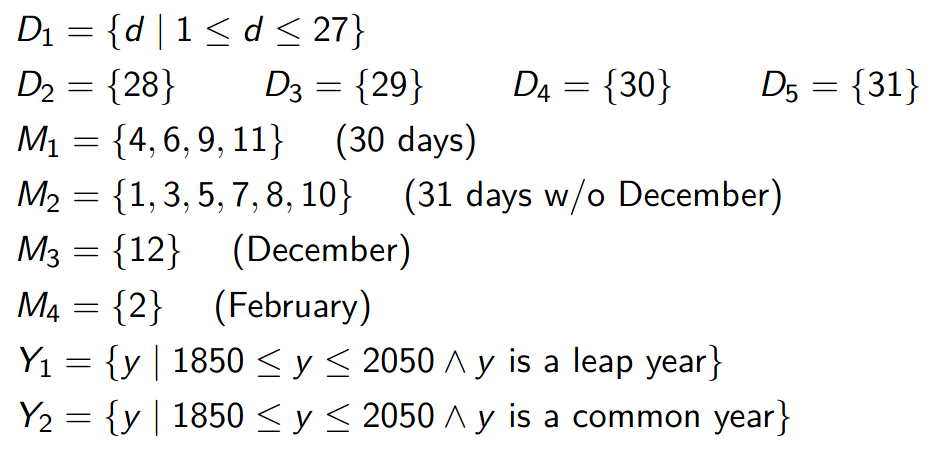
\includegraphics[width=\textwidth]{figures/descision_table_1.png}
    \end{minipage}
    \begin{minipage}{.49\textwidth}
        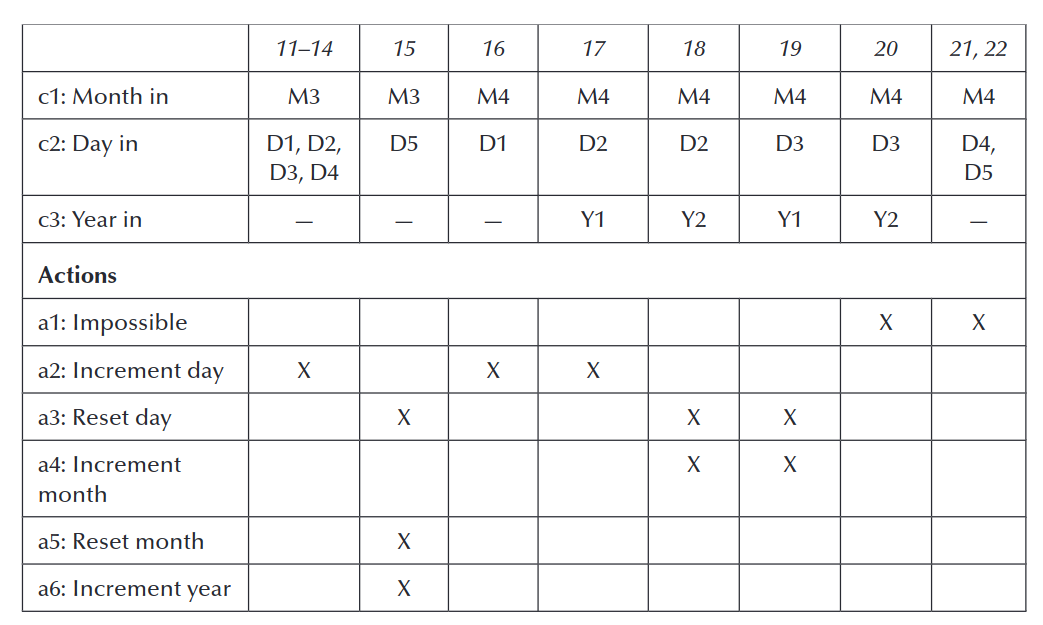
\includegraphics[width=\textwidth]{figures/descision_table_2.png}
    \end{minipage}
\end{frame}

% ------------------------------------------------------
%                       Topic 2
% ------------------------------------------------------

\begin{frame}{\mf{Topic 2: White-Box Testing}}
    > Goals\\
\end{frame}

\begin{frame}{\rf{Goals of White-Box Testing}}
    Finding specifications we've failed to do\\
    Finding specifications we've done incorrectly
\end{frame}

\begin{frame}{\rf{IMP}}
    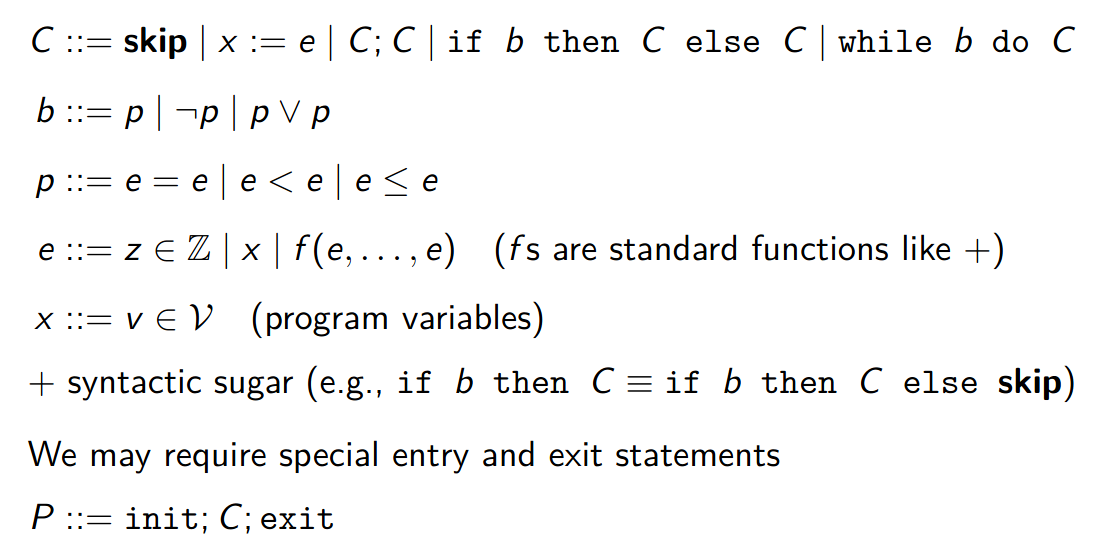
\includegraphics[width=\textwidth]{figures/IMP.png}
\end{frame}

\begin{frame}{\rf{Control Flow Graphs}}
    \tiny
    \begin{minipage}{.35\textwidth}
        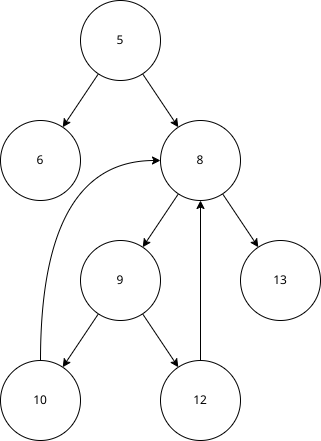
\includegraphics[width=\textwidth]{figures/control-flow.drawio.png}
    \end{minipage}\hspace{.04\textwidth}
    \begin{minipage}{.60\textwidth}
        \lstinputlisting[language=python]{code/coverage.py}
    \end{minipage}
\end{frame}

\begin{frame}{\rf{Code Coverage}}
    \lstinputlisting[language=python]{code/coverage.py}
    \tiny \texttt{python program.py \color{green}3 4 5 6 7 8 9}\\
    \tiny \texttt{python program.py \color{green}199 \color{red} 200 201 202 203}\\
    \tiny \texttt{python program.py \color{blue} abc}
\end{frame}

% ------------------------------------------------------
%                       Topic 3
% ------------------------------------------------------

\begin{frame}{\mf{Topic 3: Mutation Testing}}
    Goal? we want to test whether our test suite can detect intentional faults\\
    if it can't detect an intentional fault, we can't verify it can detect a real fault
\end{frame}

\begin{frame}{\rf{Mutation Example}}
    \begin{minipage}{.45\textwidth}
        \begin{table}
            \tiny original.py
            \lstinputlisting[language=python]{code/original.py}
        \end{table}
    \end{minipage}
    \hspace{.05\textwidth}
    \begin{minipage}{.45\textwidth}
        \begin{table}
            \tiny mutation1.py
            \lstinputlisting[language=python]{code/mutation1.py}
        \end{table}
    \end{minipage}
    
    \begin{minipage}{.45\textwidth}
        \begin{table}
            \tiny mutation2.py
            \lstinputlisting[language=python]{code/mutation2.py}
        \end{table}
    \end{minipage}
    \hspace{.05\textwidth}
    \begin{minipage}{.45\textwidth}
        \begin{table}
            \tiny mutation3.py
            \lstinputlisting[language=python]{code/mutation3.py}
        \end{table}
    \end{minipage}
\end{frame}

\begin{frame}{\rf{Mutation Score}}
    > $M_k$: failed mutants\\
    > $M_t$: total mutants\\
    > $M_e$: equivalent mutants (to original)\\
    \begin{equation}
        \frac{M_k}{M_t-M_e}
    \end{equation}
    Previous slide: $\frac{2}{3-1} = 1$
\end{frame}

% ------------------------------------------------------
%                       Topic 4
% ------------------------------------------------------

\begin{frame}{\mf{Topic 4: Data-flow Testing}}
    Usually caught at compile time\\
    Runtime errors in interpreted languages
\end{frame}

\begin{frame}{\rf{CF Graphs: Two types of nodes}}
    DEF: a variable is defined or initialized, use can be valid after\\
    USE: uses a variable, if its not defined it is a fault\\
    P-use: Predicate use, use within a predicate\\
    C-use: Condition use, use within an assignment
\end{frame}

\begin{frame}{\rf{Example}}
    \begin{minipage}{.45\textwidth}
        DEF(a, 1)\\
        DEF(b, 2)\\
        DEF(c, 3)\\
        DEF(e, 4)\\
        \vspace{10pt}\\
        USE(a, 6)\\
        USE(b, 6)\\
        USE(c, 6)\\
        USE(d, 6)\\
    \end{minipage}
    \hspace{.05\textwidth}
    \minip{.45\textwidth}{\lstinputlisting[language=python]{code/DU.py}}
\end{frame}

\begin{frame}{\rf{DU-path}}
    \begin{minipage}{.45\textwidth}
    > The path of DEF and USE from node n to node m\\
    > 3 to 5 is impossible\\
    > \texttt{p1: <1,2,5>}\\
    > \texttt{p2: <1,2,3,4,8>}

    \end{minipage}
    \minip{.45\textwidth}{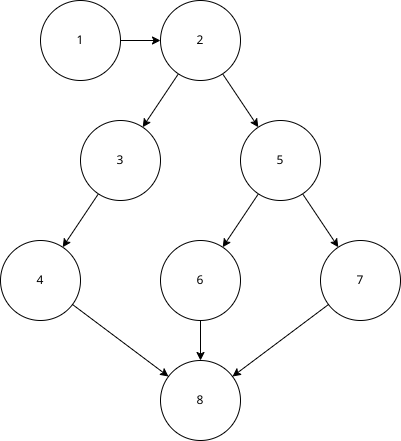
\includegraphics[width=\textwidth]{figures/du-path.drawio.png}}

\end{frame}

\begin{frame}{\rf{Slicing}}
    Instead of analyzing the entire program, its useful to split a program into small slices:

    \minip{.30\textwidth}{\centering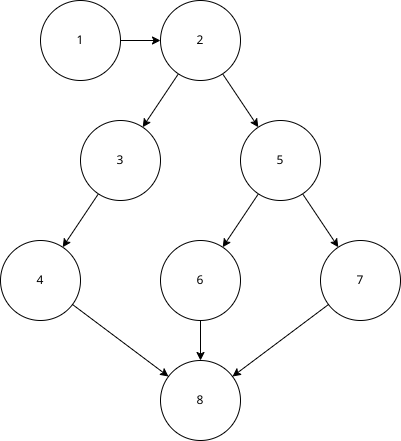
\includegraphics[height=\textwidth]{figures/du-path.drawio.png}\\\tiny original}
    \minip{.30\textwidth}{\centering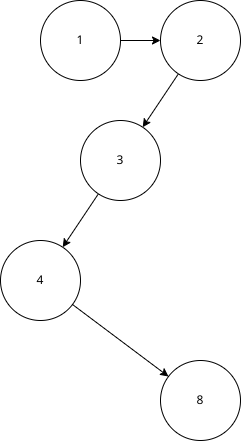
\includegraphics[height=\textwidth]{figures/slice1.drawio.png}\\\tiny slice 1}
    \minip{.30\textwidth}{\centering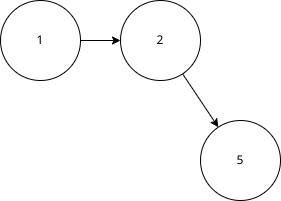
\includegraphics[height=.5\textwidth]{figures/slice2.drawio.png}\\\tiny slice 2}
\end{frame}

% ------------------------------------------------------
%                       Topic 5
% ------------------------------------------------------

\begin{frame}{\mf{Topic 5: Model-based Testing (+LCT?)}} % or Life-cycle testing
    Automatic tests!\\
    > Systematically choose a model (a design of the system) and implement it\\
    > Identify test cases and implement them\\
    > Test on the system, modify the model and repeat until the model satisfies the specification
\end{frame}

\begin{frame}{\rf{Types of models}}
    > Structural model \color{gray} e.g. class diagram\\
    \color{black}> Behavioral model \color{gray} e.g. state machine
\end{frame}

\begin{frame}{\rf{Good/bad practices in MBT}}
    > A weak model is a model which doesn't cover the important aspects of the system\\
    > A strong model is a model which may be too complex and cause unneccesary development time.\\
    These two dictate neccessity and sufficiency of the model
\end{frame}

\begin{frame}{\rf{Life-cycle testing}}
    Types:\\
    > Waterfall model\\
    > Agile development\\
    > Extreme programming\\

    \minip{.30\textwidth}{\tiny Waterfall\\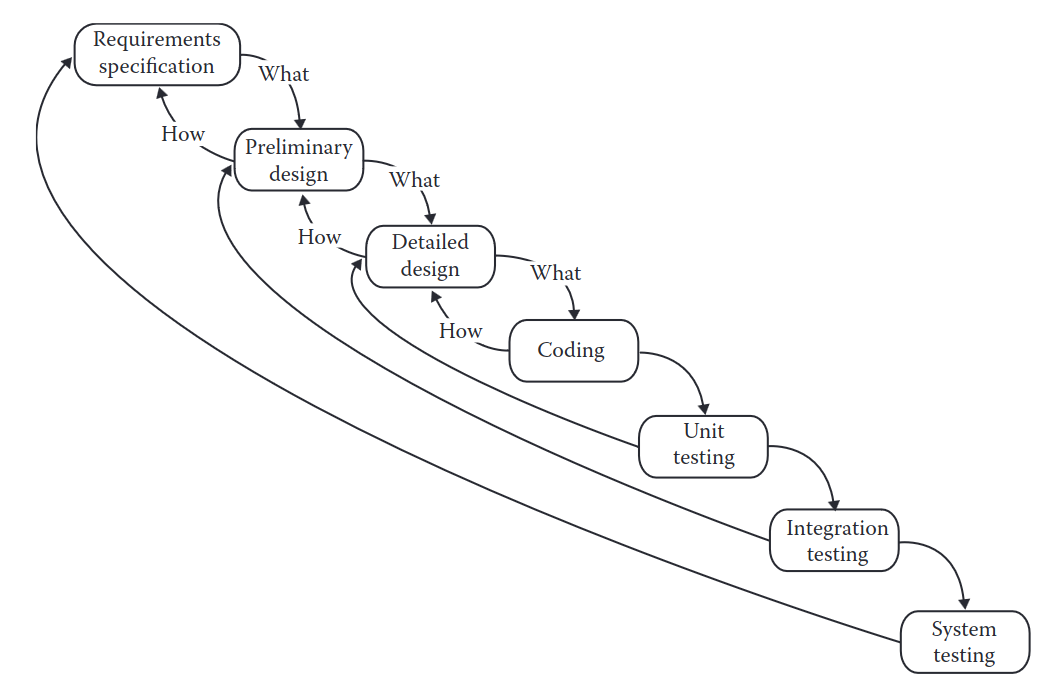
\includegraphics[height=.6\textwidth]{figures/waterfall.png}}
    \minip{.30\textwidth}{\tiny Agile\\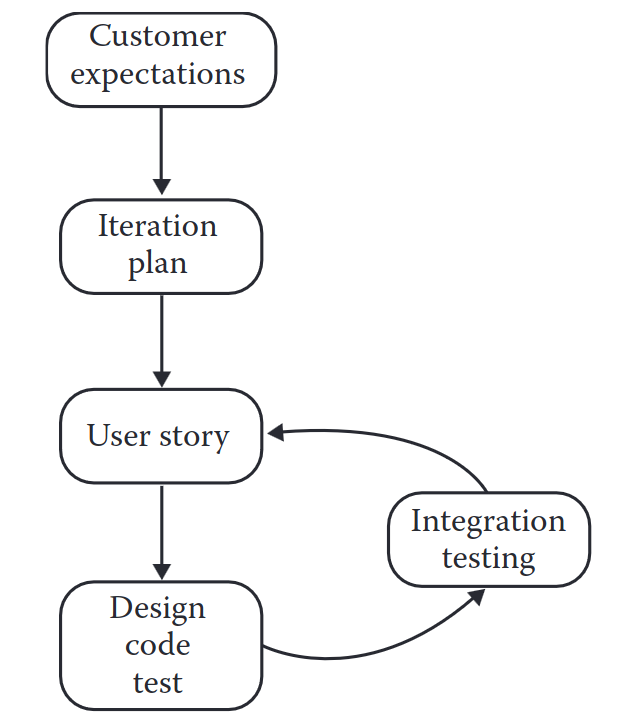
\includegraphics[height=.6\textwidth]{figures/agile.png}}
    \minip{.30\textwidth}{\tiny Extreme\\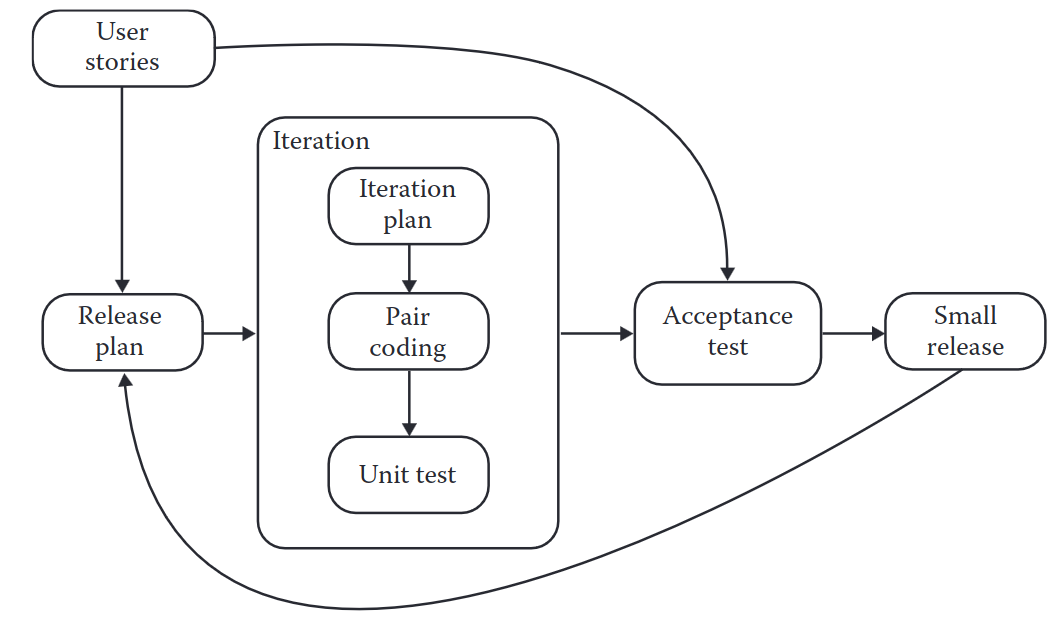
\includegraphics[height=.6\textwidth]{figures/extreme.png}}
\end{frame}

\begin{frame}{\rf{Test-driven development}}
    Writing code to fulfil tests\\
    The tests are the requirements
\end{frame}

% ------------------------------------------------------
%                       Topic 6
% ------------------------------------------------------

\begin{frame}{\mf{Topic 6: Hoare logic \& Hoare Calculus}}
    First topic in Verification\\
    What is the goal of verification?\\
    > to evaluate the correctness of the code. A more static set of methods than test.\\
    What is the difference between Hoare logic and Hoare calculus?
\end{frame}

\begin{frame}{\rf{Hoare Logic}}
    Hoare Triples\\
    Syntax: \{$\phi$\}C\{$\psi$\}\\
      VALID\\
      > \{$i>j$\} $i:=i+1$; $j:=j+1$ \{$i>j$\}\\
      > True\\
      INVALID\\
      > \{$i>=0$\} $i:=i+j$ \{$i>=0$\}\\
      > False, $j=-1$, $i=0$,    $i=0+(-1) \neq 0$

\end{frame}

\begin{frame}{\rf{Invariants}}
    variable $\theta$ is invariant if the triple \{$\theta$\}C\{$\theta$\} holds\\
    variable $\theta$ is loop invariant if while the loop is active, $\theta$ evaluates to true
\end{frame}

\begin{frame}{\rf{Hoare Calculus: seq}}
    if we have two triples, and the second takes the output of the first, this rule applies
    \begin{equation}
        \frac{\{\phi\}C_1\{\theta\} \{\theta\}C_2\{\psi\}}{\{\phi\}C_1;C_2\{\psi\}}
    \end{equation}
\end{frame}

\begin{frame}{\rf{Hoare Calculus: while}}
    this rule basicly just means checking a boolean expression before or after a loop is equivalent if the negation is checked after:
    \begin{equation}
        \frac{\{\theta\land b\}C\{\theta\}}{\{\theta\}\text{while b do}\{\theta\}C\{\theta\land\lnot b\}}
    \end{equation}
\end{frame}

% ------------------------------------------------------
%                       Topic 7
% ------------------------------------------------------

\begin{frame}{\mf{Topic 7: Weakest Precondition}}
    Strengthening preconditions in hoare calculus\\
    Take skip for example:\\
    $\frac{}{\{\phi\}skip\{\psi\}}$\\
    $\phi$ is redundant:\\
    $\frac{}{\{\phi\}skip\{\psi\}}\text{if} \phi \rightarrow \psi$
\end{frame}

\begin{frame}{\rf{Strengthening seq}}
    \begin{equation}
        \frac{\{\phi\}C_1\{\theta\} \{\theta\}C_2\{\psi\}}{\{\phi\}C_1;C_2\{\psi\}}
    \end{equation}

    \begin{equation}
        \frac{\{\phi_1\}C_1\{\phi_2\} \{\phi_2\}C_2\{\psi\}}{\{\phi\}C_1;C_2\{\psi\}}\phi \rightarrow \phi_1
    \end{equation}
\end{frame}

\begin{frame}{\rf{Strengthening while}}
    \begin{equation}
        \frac{\{\theta\land b\}C\{\theta\}}{\{\theta\}\text{while b do}\{\theta\}C\{\theta\land\lnot b\}}
    \end{equation}

    \begin{equation}
        \frac{\{\theta\land b\}C\{\theta\}}{\{\theta\}\text{while b do}\{\theta\}C\{\theta\land\lnot b\}} \phi \rightarrow \theta \text{ and } \theta \land \lnot b \rightarrow \psi
    \end{equation}

\end{frame}

% ------------------------------------------------------
%                       Topic 8
% ------------------------------------------------------

\begin{frame}{\mf{Topic 8: Bounded Model Checking}} % or Bounded-model checking or Interval analysis
    Motivation: verifying a program with a single path has a single path\\
    > A program with branches has finite paths\\
    > A looping program has infinite paths\\
    Unrolling a CFG with a loop\\
    > We add a bound, a finite number of loops

\end{frame}

\begin{frame}{\rf{Unrolling a CFG}}
    \minip{.45\textwidth}{\lstinputlisting{code/bounded-model1.txt}}
    \hspace{.05\textwidth}
    \minip{.45\textwidth}{\lstinputlisting{code/bounded-model2.txt}}

    postcondition should only hold after the predicate becomes false (last iteration)
\end{frame}

\begin{frame}{\rf{Unrolling a CFG}}
     \minip{.45\textwidth}{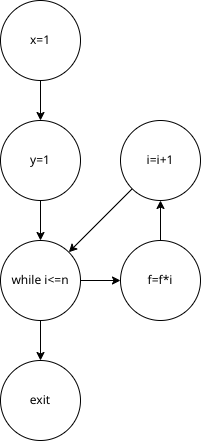
\includegraphics[height=\textwidth]{figures/unrolling1.drawio.png}}
     \minip{.45\textwidth}{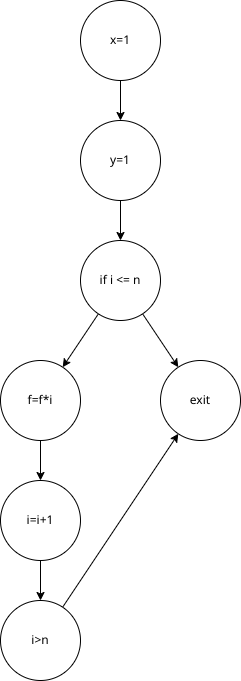
\includegraphics[height=\textwidth]{figures/unrolling2.drawio.png}}
\end{frame}

\begin{frame}{\rf{Static single assignment}}
    instead of changing the value of a variable, we make a new variable at every assignment.\\
    consider the following code:\\
    \lstinputlisting{code/single-assignment.txt}
\end{frame}


\end{document}